% INSTRUCTIONS:
% To compile this file, run "latex HW_example";  you need to do it TWICE
%    to get the cross-references (to equations, etc) to show correctly.
% Figures can be included as shown below.  If you don't have a figure,
%    comment out those lines using % signs at the beginning of each line,
%    or else just keep hitting RETURN when LaTeX gives an error message
%    saying that it can't find the figure file.
% Run "dvips HW_example.dvi" to make a Postscript file HW_example.ps,
%    and then "ps2pdf HW_example.ps" to make a PDF file HW_example.pdf.

\documentclass[12pt]{article}
\usepackage{graphicx,indentfirst}

\pagestyle{plain}
\baselineskip 18pt
\textwidth 6.5in
\textheight 7.8in
\oddsidemargin 0.1in
\evensidemargin 0.1in
\topmargin 0.3in

\newcommand{\be}{\begin{equation}}
\newcommand{\ee}{\end{equation}}
\newcommand{\reff}[1]{(\ref{#1})}


\begin{document}

\title{Computational Physics \\ Homework 1}
\author{Yi-Hsuan Hsu}
\date{09/11/2014}
\maketitle


\section{Problem 1}

Calculating integration using recursion relationship. 

\begin{equation}
%a^2 + b^2 = c^2 = c_2 = \int f(x) dx
I_n = \frac{1}{n} - 5I_{n-1}
\end{equation}

\subsection{Algorithms}

Single-precise(32 bit) floating point number can be assigned by np.float32(). Double-precise floating point number are default in Python. Put initial single and double precise number into simple loop recursion function. Stop at given number of N (here N=30)\ and return final result into array.

Exact solution could be solved by Python integration function integrate.quad(). Integrate.quad would return integration and estimating error. 

\subsection{Description of program}

It's a simple practice for new python user as I am. Well organized structure and comment keep it clear to review. Variable are well named as it represent.

\subsection{Sample output}

Error analysis as below

\begin{eqnarray}
&I_{exact} = I_{approx.} + \epsilon\\
&I_N = \frac{1}{N} - 5*I_{N-1} \pm 5^N*\epsilon
\end{eqnarray}

Where we can estimate the error of numerical approximation. 

Single-precise input return good approach till N=7, error become bigger and bigger after. Interesting things is that N=11 return the first negative number, which is the same order as professor's Example 2. Afterward, the number jump positive and negative term by term, which is expected from the recursion equation. Finally, N=30 returns error up to tenth of twelve, roughly consists with (6). On the last two columns shows the error compare to exact number, which also confirmed that error multiple 5 at each recursion.

\begin{figure}[h]
\begin{center}
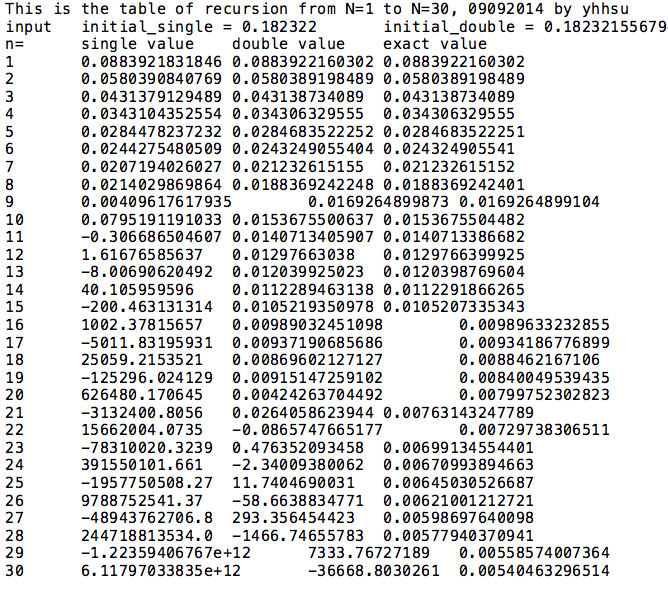
\includegraphics[width=0.4\textwidth]{result.png}
\caption{Result table snapshot.}
\label{fig1}
\end{center}
\end{figure}

Double-precise input, in the other hand, performs well till N=18. Obviously performs much better than single precise floating point number.

The build-in integration function gives the same number as professor's example from Mathematica. Numerical computation returns error within ten powered sixteenth precision. 


\section{Problem 2}

Find numerical approximation of the bridge height to 5 significant digits.

\subsection{Theory}
\begin{figure}[h]
	\begin{center}
		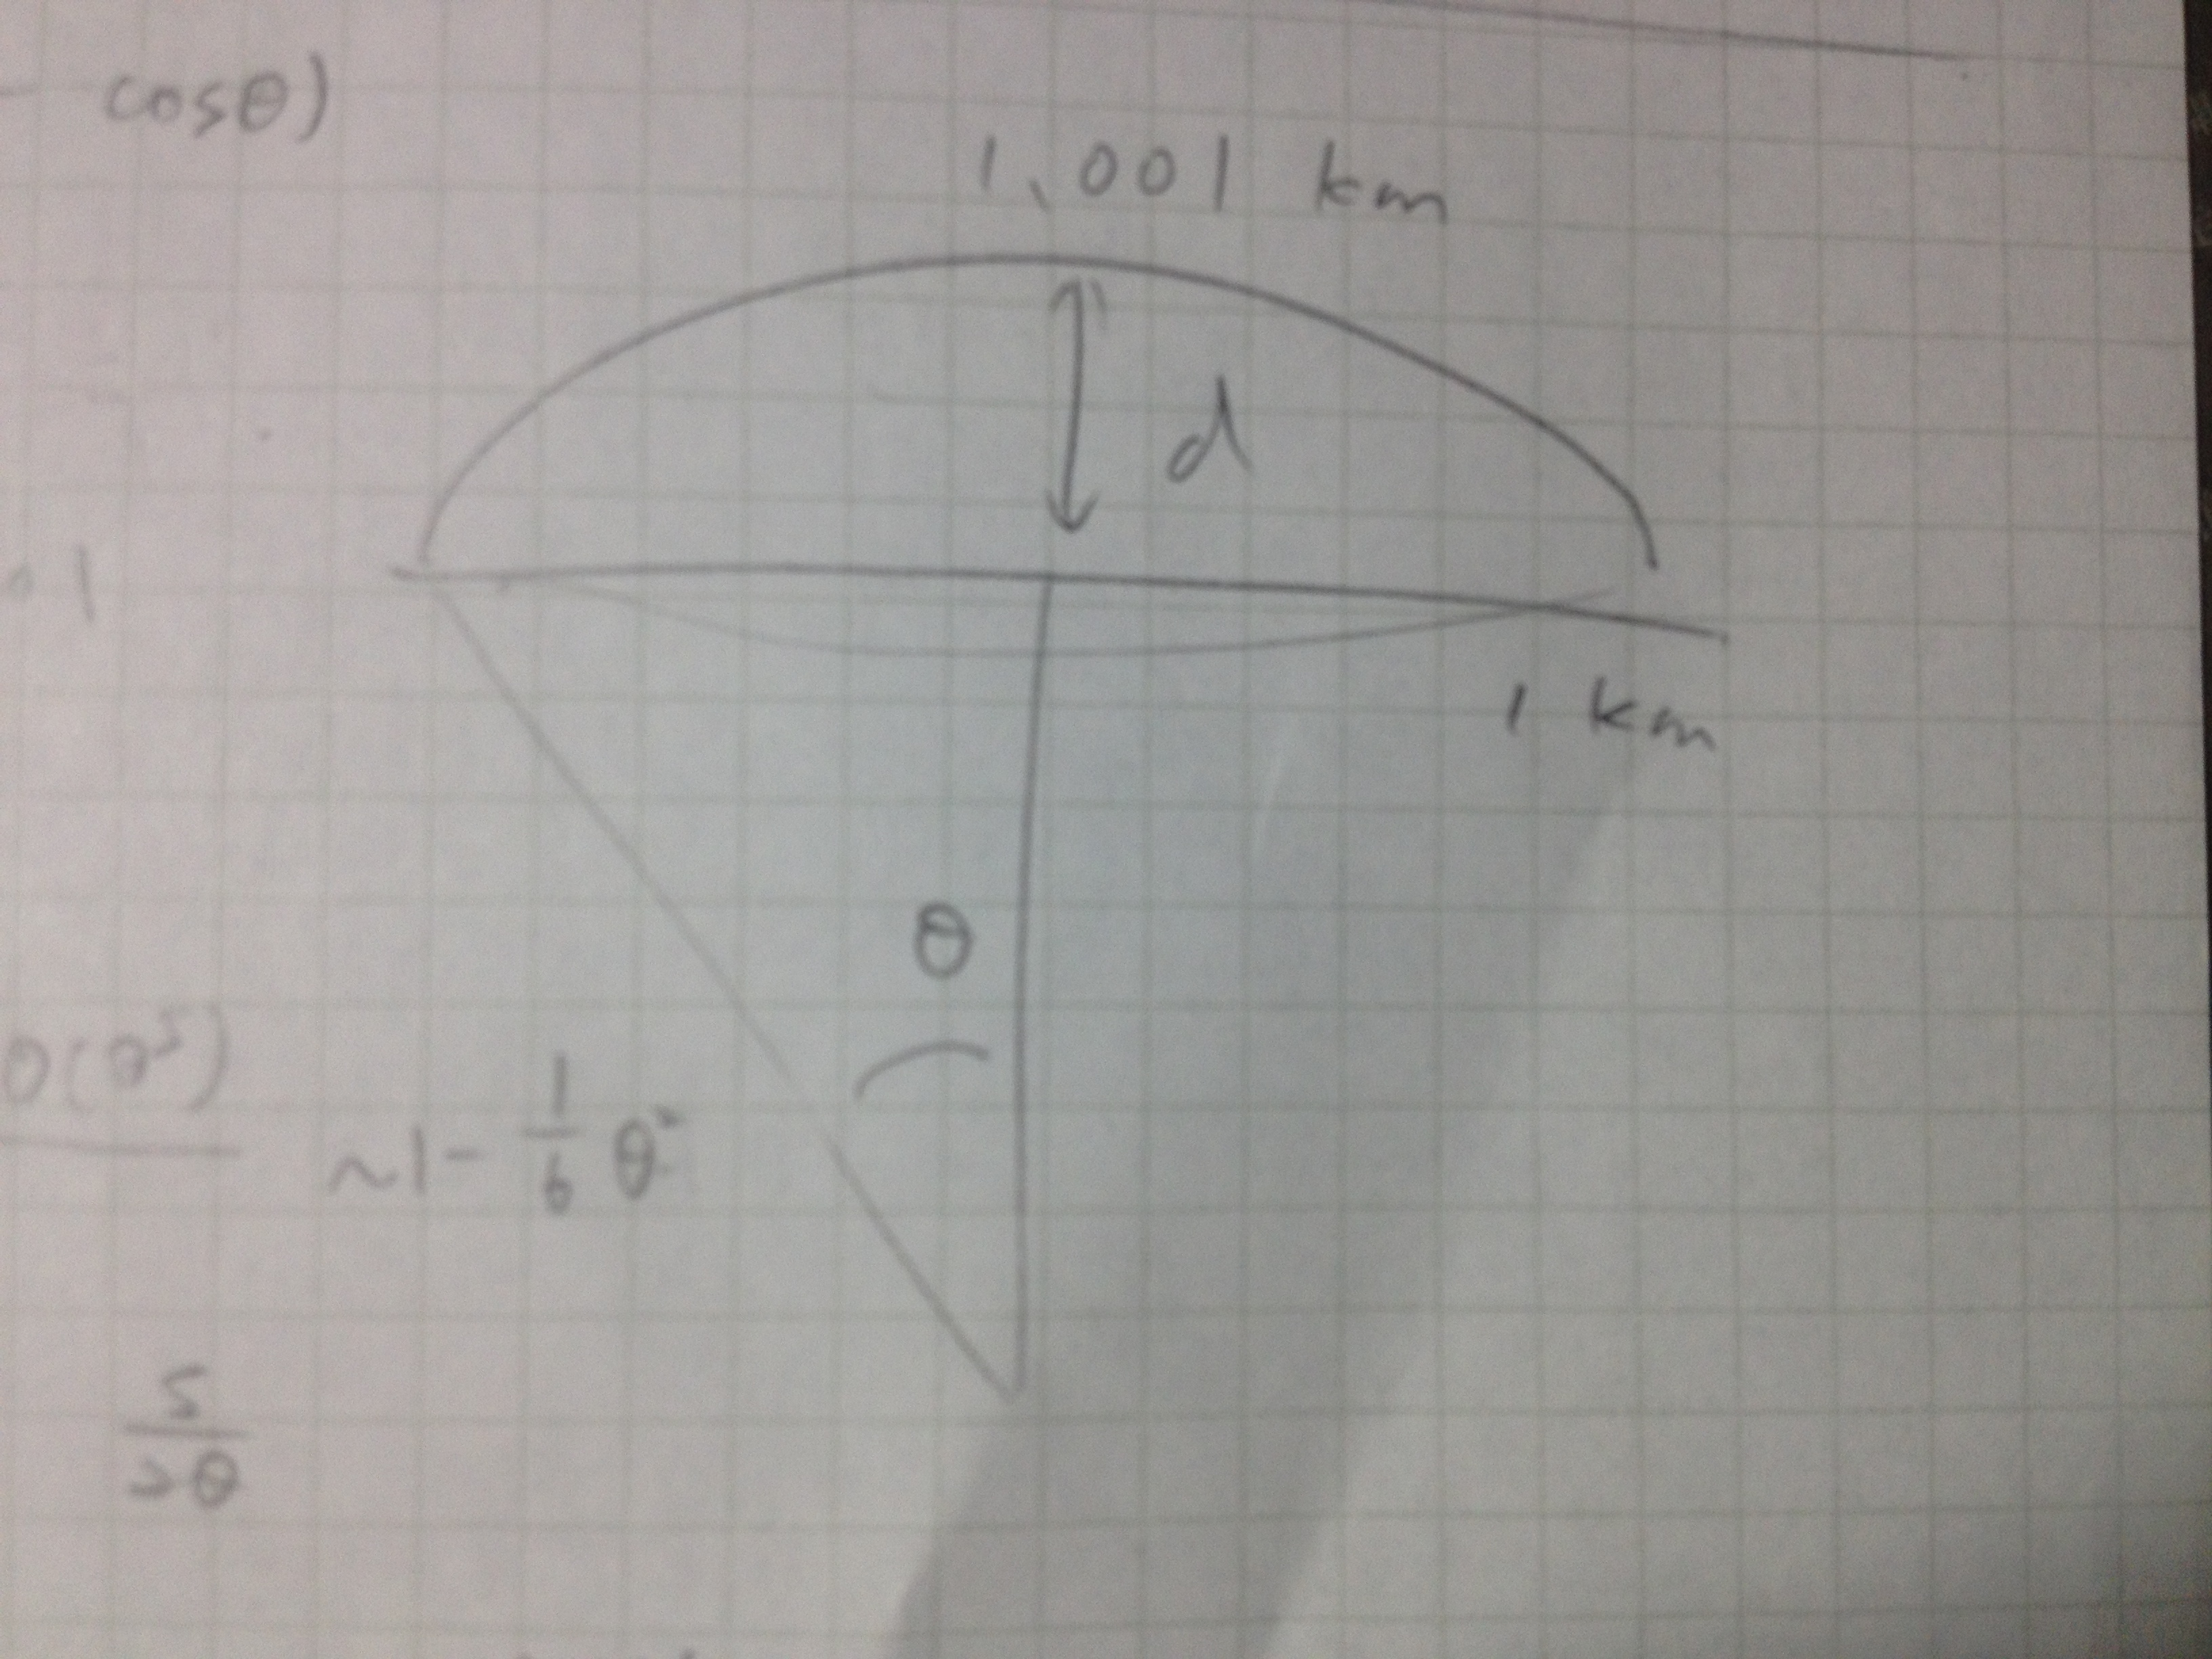
\includegraphics[width=0.4\textwidth]{problem2}
		\caption{Picture and variables.}
		\label{fig2}
	\end{center}
\end{figure}
\subsection*{Method.1}
Consider the upper fan-shaped area as a triangle. Therefore, the bridge height d simply equal square root of arc square minus distance square.

\begin{eqnarray}
d  = \sqrt{0.5005^2 - 0.5^2}   = 0.022366
\end{eqnarray}
\subsection*{Method.2}
\begin{eqnarray}
&d = r-rcos(\theta)=r(1-cos(\theta))\\
&L = 2rsin(\theta)\\
&S = 2r\theta
\end{eqnarray}
From (2) and (3), we have
\begin{eqnarray}
	\frac{L}{S}=\frac{sin(\theta)}{\theta}
\end{eqnarray}
Using Taylor expansion of Sin,

\begin{eqnarray}
Sin\theta=\theta-\frac{1}{6}\theta^3+\varepsilon(\theta^5)
\end{eqnarray}
Ignoring the error term, (8) can be rearrange to 
\begin{eqnarray}
\theta=\sqrt{6(1-\frac{L}{S})}
\end{eqnarray}
Finally, Combining (5)(7)(10) we have
\begin{eqnarray}
d = \frac{S}{\theta}(1-cos(\theta))=0.019364
\end{eqnarray}

\subsection{Discussion}
Obviously, Method.1 do not approach to the answer very well. While Method.2 using Taylor expansion, the error term depends on theta powered five. In this case, theta is as small as 0.077421. Therefore I could expect that the result is within 5 significant digit precision.


\end{document}
